%
% main.tex -- Paper zum Thema Machine Learning und Klimamodelle
%
% (c) 2018 Hochschule Rapperswil
%
\tikzstyle{inputNode}=[draw,circle,minimum size=10pt,inner sep=0pt]
\tikzstyle{stateTransition}=[-stealth, thick]

\chapter{Machine Learning und Klimamodelle\label{chapter:learning}}
\lhead{Machine Learning und Klimamodelle}
\begin{refsection}
\chapterauthor{Martin Stypinski}
	
	


	Machine Learning ist vermutlich eines der grossen Schlagworte des vergangenen Jahres. Mit Machine Learning wird vermutet, dass die grossen Mustererekennungs und Datenprobleme unserer Zeit gelöst werden können. Sei es die Erkennung von Schrift und Bild, die Erkennung von Sprache oder die Erkennung einer Anomalie. Weiter sollen, bis zu einem gewissen Grad, Vorhersagen auf bestehenden Daten getroffen werden, welche einen nicht trivialen Zusammenhang aufweisen oder nicht vollständig Deterministisch sind (z.B Börsenkurse, Wetter, o.a). In dieser Arbeit wird speziell auf Neuronale Netzwerke mit geringer Tiefe eingegangen, diese dafür versucht detailiert nachzuvollziehen.
	

	Im Gegensatz zur Wettervorhersage mit entwickelten Modellen ist es mittels künstlicher neuronaler Netzwerke (KNN) möglich ein Art Blackbox zu trainieren und später zu verwenden. Die Parameter erlernt das System selbst und kann anhand dieser trainierten Parameter eine Vorhersage treffen. Mit einer grosszügigen Datengrundlage ist das System im Stande viel bessere Lösungen zu approximieren als mit einfacheren Modellen möglich ist. Allein dieser Umstand ist ein treibender Faktor um anspruchsvolle Probleme mittels diser Methode zu lösen. Ist die Datengrundlage gross genug, so kann das System sehr gute Lösungen approximieren.
	
	Das Wetter eignet sich sehr um Vorhersagen mittel Machine Learning zu treffen. Es existieren genug freie Daten und es können Schlüsse auf bereits bestehende Modelle gezogen werden. Dies wurde auch durch Grover et al. gezeigt. %(Insert Paper here: http://erichorvitz.com/weather_hybrid_representation.pdf)
	Aus wissenschaftlicher Sicht mag es interessant sein, grosse Modelle und bessere Vorhersagen zu bauen, aus lerntechnischer Sicht wird aber an dieser Stelle bewusst ein sehr kleines Modell erarbeitet. Dieses Modell soll aber möglichst die tieferen Konzepte aufzeigen, welche diese Methode so erfolgreich macht.
	
	\section{Die Wärmeleitungsgleichung als diskretes ML Problem}
	Die Wärmeleitungsgleichung (gem. Kapitel xyz) ist eine partielle Differential Gleichung welche für diesen Anwendungszweck in einer Dimension gemäss Gleichung \ref{eq:waermeleitung-1d} beschrieben werden kann.
	\begin{equation}
	\frac{\partial T}{\partial t} = \kappa \frac{\partial^2}{\partial x^2} T
	\label{eq:waermeleitung-1d}
	\end{equation}
	Das gewählte Model soll eine Vorhersage über die Zeit machen können. Sowohl die Zeit als auch der Ort wird diskretisiert und der Zeitschritt $T(x,y) \rightarrow T(x,t+1)$ erlernt. An dieser Stelle soll erwähnt, dass die Lösung mathematisch diskretisiert lösbar ist - dieser Umstand wird später ausgenutzt um Trainingsdaten zu erzeugen. Um die diskrete Lösung verständlich herzuleiten wird das Modell eines Stabs $S$ (1D) genommen. Der Stab wird nun unterteilt in $N+2$ äquidistante Punkte, wobei am Anfang und am Ende des Stabes die Temperatur fix ist. Es existieren folglich $S(x_0, \dots, x_{N+1})$ Punkte und folglich gilt: $x_0 = a$, $x_{N+1} = b$. Die Lösung kann nun über die 2. Abbleitung angegangen werden:
		
	\begin{align}
	T_{x}(x, t)  &= \frac{T(x-\frac{1}{2}h, t) - T(x+\frac{1}{2}h, t)}{h} \\
	T_{xx}(x, t) &= \frac{T_{x}(x-\frac{1}{2}h, t) - T_{x}(x+\frac{1}{2}h, t)}{h} \\
				 &= \frac{\frac{T(x-h, t) - T(x+h, t)}{h} - \frac{T(x, t) - T(x+1,t)}{h}}{h} = \frac{T(x-h, t) - 2 T(x, t) + T(x+h, t)}{h^{2}}
	\end{align}
	
	Aus der Initialen Beziehung lässt sich folglich herleiten:
	
	\begin{equation}
	T(x,t) \rightarrow T(x,t+1) : T(x,t+1) = \frac{\kappa}{h^{2}} T(x-h,t) - 2 \cdot T(x,t) + T(x+h,t)
	\end{equation}
	
	Aus der Herleitung der Gleichung wird schnell ersichtlich, was die menschliche Intuition vermuetet. Die punktuelle Hitze in einem Stab breitet sich sowohl nach Rechts als auch nach Links aus. Der nächste Zeitschritt ist abhänig von den benachbarten Punkten. Dies ist eine Näherung, mit welcher das Netz trainiert werden kann. Eine passende Machine Learning Blackbox soll anhand 3 diskreter Punkte die Temperatur am mittleren Punkt im nächsten Zeitschritt berechnen.
	\begin{figure}[h]
		\centering
		
		\begin{tikzpicture}[
		node distance = 4mm and 22mm
		]
		\node (adc) [draw,minimum size=18mm] {Black Box Solver};
		%
		\coordinate[above left = of adc.west]   (a1);
		\coordinate[below = of a1]              (a2);
		\coordinate[below = of a2]              (a3);
		\coordinate[above right= 8mm and 22mm of adc.east]  (b1);
		\foreach \i [count=\xi from 1] in {2,...,5} 
		\coordinate[below=of b\xi]  (b\i);
		%
		
		\foreach \i [count=\xi from 1] in {$X_{n-1,t}$,$X_{n,t}$,$X_{n+1,t}$}
		\draw[-latex']  (a\xi) node[left] {\i} -- (a\xi-| adc.west);
		
		\foreach \i [count=\xi from 3] in {$X_{n,t+1}$}
		\draw[-latex'] (adc.east |- b\xi) -- (b\xi) node[right] {\i};
		\end{tikzpicture}
		\label{fig:mst_blackBoxSolver}
		\caption{BlackBox Solver}
	\end{figure}
	
	\subsection{Neuronales Netzwerk - Die Blackbox}
	
	Der Gedanke, dass die Blackbox mit einem Neuronalen Netzwerk ersetzt werden kann ist sehr naheliegend. Bei künstlichen Neuronalen Netzwerken (KNN) handelt es sich um eine sogenante Supervised Learning Methode. Diese benötigen zuerst eine Trainingsphase mit bestehenden Datensätzen um die inneren Parameter zu 'erlernen'. Zu einem späteren Zeitpunkt kann Anhand der Parameter das erlernte wiedergegeben werden. Ein KNN besteht aus vielen einzelnen Neuronen die zusammen das Netzwerk bilden. Wie aus Abbildung \ref{fig:mst_neuronalnetwork} entnommen werden kann, ist ein einzelnes Neuron eine gewichtete Summe mit Bias Parameter ($b$), zur Brechung der Linearität des Systems werden sogenante Aktivierungsfunktionen ($\sigma$) verwendet. Diese Funktion wird benötigt, damit das Netzwerk nicht eine linear Kombination von vielen Neuronen ist und somit verinfacht zu einer einfachen Funktion werden kann. Die Neuronen werden in Gruppen angeordnet, welche oft als \textit{Input Layer}, \textit{Hidden Layer} und \textit{Output Layer} bezeichnet werden. 
	
	\begin{figure}[h]
		\centering
		\input{learning/neuronal_network.tex}
		\label{fig:mst_neuronalnetwork}
		\caption{Neuronales Netzwerk}
	\end{figure}
	
	Die Trainingsphase besteht im Grunde aus 3 einfachen Schritten und kann mithilfe eines Beispiel Datensatzes erklärt werden. Der Datensatz $D$ enthält viele Input Vektoren $I_n$ und dazu die passnden Output Vektoren $O_n$. Jeweils ein Vektor $I$ und $O$ bilden zusammen ein Paar welches die Abbildung innerhalb des Neuronalen Netzes trainieren soll. Am Beispiel der Wärmeleitungsgleichung entspricht $I_n = (T(x_{n-1}, t), T(x_{n}, t), T(x_{n+1}, t))$ und $O_n = T(x, t_{n+1})$. Weiter sollen während der Trainingsphase alle inneren Parameter $w_{i}, b_{i}$ trainiert werden. (vgl. Abbildung \ref{fig:mst_neuronalnetwork}).
	\begin{enumerate}
		\item {\textbf{Ausbreitung:} Für ein gegebenes $I_{n}$ wird mittels der inneren Parameter $w_{i}, b_{i}$ ein Output $O'_{n}$ berechnet. Sofern keine inneren Parameter gesetzt sind, so werden diese randomisiert oder mit einer 'inteligenten' Methode initialisiert.}
		\item {\textbf{Fehler Berechnung:} Der Fehler zwischen dem berechneten Output $O'_{n}$ und dem erwarteten Output $O_{n}$ wird berechnet. Für die Fehlerberechnung wird eine sogenante loss-Funktion verwendet. Oft wird an dieser Stelle die mittlere quadratische Abweichung (mean-squared error) verwendet. Im gezeigten Beispiel wurde der relative Fehler verwendet, um den Fehler unabhänig des Wertebereichs zu halten.}
		\item{ \textbf{ Fehlerrückführung:} In diesem Schritt wird mittels Gradientenabstiegsverfahren (oder ähnlich) versucht der Fehler auf den Daten zu minimieren. Dafür werden die inneren Parameter des Netzes angepasst. In dem hier gezeigten Beispiel wurde davon abgesehen mit anderen Methoden zu experimentieren und es wurde ein einfacher Gradientenabstieg verwendet.}
	\end{enumerate}
	Das Ziel des Trainings ist es so lange zu trainieren und diese Schritte zu wiederholen bis die loss-Funktion so klein wie möglich ist. Die loss-Funktion sollte gegen einen Wert konvergieren, jedoch niemals 0 erreichen. Dies wäre ein Indikator dafür, dass das Netz überparametrisiert ist oder aber die Netzgrösse für das gegebene Problem zu gross. Dies wird auch in der Literatur als Overfitting bezeichnet.
	
	
	\subsection{Trainingsdaten \& 'Faire' Kurven}
	Mit dem Verständnis für neuronale Netzwerke müssen nun die Daten erschaffen werden um das Netzwerk zu trainieren. Da das Netzwerk dazu neigt 'Trivialitäten' zu lernen wurden an die Datengenerierung einige Kriterien gestellt. Der Erwarungswert sollte möglichst 0 sein, damit die die Variable $b$ keinen Offset hat. Weiter sollen Kurven mit unterschiedlichsten Krümmungen erzeugt werden, damit soll sichergestellt werden können, dass keine anderen numerischen Effekte gelernt werden. Als besonders hilfreich haben sich hier die Hermite-Polynome erwiesen.
	
	\begin{align}
		H_{n}(x) &=(-1)^{n}e^{x^{2}}{\frac {\mathrm {d} ^{n}}{\mathrm {d} x^{n}}}e^{-x^{2}} \\
		H_{n}(x) &=(-1)^{n}\sum _{k_{1}+2k_{2}=n}{\frac {n!}{k_{1}!k_{2}!}}(-1)^{k_{1}+k_{2}}(2x)^{k_{1}}
	\end{align}
	
	Die ersten 5 Hermite Polynome sind in einfacher Schreibweise folgende:
	
	\begin{align}
	H_{0}(x) &= 1\\
	H_{1}(x) &= 2x\\
	H_{2}(x) &= 4x^{2}-2\\
	H_{3}(x) &= 8x^{3}-12x\\
	H_{4}(x) &= 16x^{4}-48x^{2}-12
	\end{align}
	
	Zur Generierung der Daten wurde ein Vektor $v=(H_0, \dots ,H_9)$ gwählt. Jeder Punkt in diesem Vektor representiert ein Hermite Polynom n-ten Grades. Dies wird benötigt um kleine Hermite Polynome zu verwenden und mittels linearkombination verscheidene Kurven zu generieren. Es soll vermieden werden, dass zu grosse Werte entstehen oder zu extreme Krümmunen entstehen daher wurde auf ein Grad über 10 abgesehen. Das Polynom 10ten Grades hat bereits $x^{10}$ was verdeutlicht wie schnell die Kurven gegen den Rand ansteigen.
	
	\begin{figure}[h]
		\centering
		\begin{tabular}{ccc}
			\includegraphics[scale=0.25]{learning/img/curves/wave0.png} &
			\includegraphics[scale=0.25]{learning/img/curves/wave1.png} &
			\includegraphics[scale=0.25]{learning/img/curves/wave2.png} \\
			
			\includegraphics[scale=0.25]{learning/img/curves/wave8.png} &
			\includegraphics[scale=0.25]{learning/img/curves/wave4.png} &
			\includegraphics[scale=0.25]{learning/img/curves/wave3.png}
		\end{tabular}
		\label{fig:mst_hermiteexample}
		\caption{Einige Beispiele von Kurven die Mittels Hermite-Polynom erzeugt wurden.}
	\end{figure}
	
	Aus den generierten Kurven werden mithilfe eines ODE-Solvers die Input und Output Daten erzeugt. Die Kurven werden diskretisiert und aus Form-Gründen in die Vektoren $I_n$ und $O_n$ aufgeteilt. Es werden pro Kurve mehrere Vektorpaare gebildet um die Daten so gut wie möglich auszunutzen. Mihilfe dieser Daten wird nun das Neuronale Netzwerk trainiert.
	
	\subsection{Netzwerk Design \& Erwartung}
	Ein KNN muss zuerst entworfen werden und einige Entscheidungen bezüglich Meta-Parametern getroffen wernde. Normalerweise stehen an dieser Stelle viele Fragen im Raum unter anderem die Anzahl Neuronen und die Anzahl Hidden Layers umfasst. In dem gewählten Beispiel der Wärmeleitungsgleichung ist die Antwort jedoch sehr naheliegend. Der Schritt $T \rightarrow T+1$ ist sehr gut dokumentiert und verstanden. Es wird ein Input Vektor der Länge 3 und ein skalrer Output benötigt. Es ist bekannt, dass mittels einer Linearen Abbildung der Output $O_n$ aus dem Input $I_n$ erzeugt werden kann. Folglich ergibt sich eine Netzwerkstruktur analog zu Abbildung \ref{fig:mst_neuronalnetworkdemo}.
	
	\begin{figure}
		\centering
		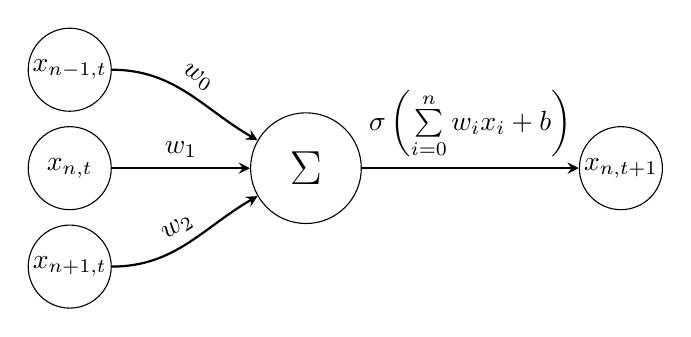
\begin{tikzpicture}
		\node[draw,circle,minimum size=40pt,inner sep=0pt] (x) at (0,0) {\LARGE $\Sigma$};
		
		\node[inputNode,minimum size=30pt] (x1) at (-3, 1.25) {$x_{n-1,t}$};
		\node[inputNode,minimum size=30pt] (x2) at (-3, 0) {$x_{n,t}$};
		\node[inputNode,minimum size=30pt] (x3) at (-3, -1.25) {$x_{n+1,t}$};
		\node[inputNode,minimum size=30pt] (x4) at (4, 0) {$x_{n,t+1}$};
		
		\draw[stateTransition] (x1) to[out=0,in=150] node [midway, sloped, above] {$w_0$} (x);
		\draw[stateTransition] (x2) to[out=0,in=180] node [midway, sloped, above] {$w_1$} (x);
		\draw[stateTransition] (x3) to[out=0,in=210] node [midway, sloped, above] {$w_2$} (x);
		\draw[stateTransition] (x) to[out=0,in=180] node [midway, sloped, above] {$\sigma \left( \sum\limits_{i=0}^{n}{w_ix_i} + b \right)$} (x4);
		\end{tikzpicture}

		\label{fig:mst_neuronalnetworkdemo}
		\caption{Einige Beispiele von Kurven die Mittels Hermite-Polynom erzeugt wurden.}
	\end{figure}
	
	Zusätzlich können einigen Restriktionen eingebaut werden:
	\begin{itemize}
		\item {\textbf{$\sigma$:} Als Aktivierungsfunktion wird eine lineare Funktion gewählt.}
		\item {\textbf{$b$: } Die Bias-Variable wird auf 0 gesetzt und während dem Training nicht verändert, es ist zu erwarten, dass $b=0$ sein muss!}
		\item {\textbf{$w_{0,1,2}$: } Die Parameter für das Gewicht werden trainiert, es könnte hier noch noch $w_0 = w_2$ in Erwägung gezogen werden, um die Symetrie auszunutzen.}
	\end{itemize}
	Das Netz hat somit 3 Parameter $w_0, w_1, w_2$ welche erlernt werden müssen. Aus der mathematischen Herleitung ist zu erwarten, dass der Gewichtsvektor $w_{0,1,2}$ die Lösungsform $w = \theta \cdot (1, -2, 1)$ annimmt. $\xi$ ist an dieser Stelle ein Platzhalter für $\xi = \frac{\kappa}{h^{2}}$ welche einfach zusammen gefasst werden können.
	
	
	Nach zahlreichen Trainingsanläufen mit unzähligen Iterationen kann festgehalten werden, dass die mathematische Herleitung genau dem erlernten des Neuronalen Netzwerks entspricht (vgl. Tabelle \ref{tbl:result_heat}) Das Tabelle enthält nur ein Beispiel welches aus dem Training hergeleitet werden konnte. Die Resutlate sind nicht deterministisch, da die Generierung der Daten randomisiert stattfindet. Wichtig ist aber, dass die Lösungsform ($w = \xi \cdot (1, -2, 1)$) stets erfüllt wurde!
	
	\begin{table}[h]
		\centering
		\def\arraystretch{1.1}
		\begin{tabular}{l|c|c}
			Parameter & Erwartung & Experiment \\
			\hline
			w & $\begin{bmatrix} 0.36 \\ -0.73 \\ 0.37 \end{bmatrix}$ & $ \xi \cdot \begin{bmatrix} 1 \\ -2 \\ 1 \end{bmatrix}$ \\
			b & 0 & 0 \\
		\end{tabular}
		\label{tbl:result_heat}
		\caption{Resultate der erlernten Wärmeleitungsgleichung.}
	\end{table}
	
	Es wurde mit einem einfachen Experiment gezeigt, dass das Lernverhalten des Neuronalen Netzwerkes anhand eines einfachen Beispiels verstanden werden kann und durchaus durchschaubar ist. Das Problem dieses Beispiels ist jedoch, dass ein KNN nicht wirklich benötigt wird, da im Grunde die Lösung numerisch einfach bestimmt werden kann.


%
% burgerintro.tex
%
% (c) 2018 Prof Dr Andreas Müller, Hochschule Rapperswil
%
\subsection{Nichtlineare Transportgleichung\label{subsection:nichtlineare}}
Die Gleichung von Burgers in der Form
\begin{equation}
\frac{\partial u}{\partial t} + u\frac{\partial u}{\partial x}=0
\qquad\text{mit Anfangsbedingung}\qquad
u(0,x) = u_0(x)
\label{burgers:transport}
\end{equation}
modelliert ein nichtlneares Transportproblem.
Die Gleichung~\eqref{burgers:transport} ist eine quasilineare partielle
Differentialgleichung erster Ordnung, die mit der Methode der
Charakteristiken \cite{burgers:pde} gelöst werden kann.
Die Charakteristiken-Gleichungen sind
\begin{align*}
t'(s)&=1
\\ 
x'(s)&=u
\\
u'(s)&=0
\end{align*}
Aus der ersten Gleichung leitet man ab, tdass $s=t$.
Die dritte Gleichung besagt, dass $u$ entlang einer Charakteristik konstant
ist, also $u(s)=u_0$.
Die zweite Gleichung besagt dann, dass die im Punkt $(0,x_0,u_0(x_0))$
beginnende Charakteristik eine Gerade mit $x(t)=x_0 + u_0(x_0)t$ ist.

\begin{figure}
\centering
\includegraphics[width=\hsize]{learning/welle.jpg}
\caption{Lösung der Gleichung von Burgers mit Hilfe der Methode
der Charakteristiken.
Die Lösungsfläche ist darstellbar als eine Schar von Geraden (gelb).
\label{burgers:charloesung}}
\end{figure}
Die Abbildung~\ref{burgers:charloesung} 
zeigt eine Lösung mit einer Gauss-Verteilung als Anfangsbedingung.
Es ist offensichtlich, dass die gezeigte Fläche früher oder später nicht
mehr Graph einer Funktion $u(x,y)$ sein kann.
Es entwickelt sich eine Sprungstelle, die Gleichung von Burgers ist
ein Modell für eine Schockwelle.
Man kann insbesondere nicht erwarten, dass die Gleichung von Burgers
für beliebige Zeiten $t$ eine glatte Lösung hat, selbst wenn die
Anfangsbedingungen glatt waren.
Man muss sich mit einer schwachen Lösung begnügen.
Dies hat sowohl auf numerische Lösungsverfahren Auswirkungen wie auch
auf das Problem, Trainingsdaten für auf Machine Learning basierenden
Lösungsalgorithmus zu erzeugen.

\subsection{Erhaltungssatz\label{subsection:erhaltungssatz}}
Die Gleichung von Burgers kann man auch in der Form
\begin{equation}
\frac{\partial u}{\partial t}
+
\frac{\partial}{\partial x} \frac{u^2}{2}
=
0
\label{burgers:erhaltungssatz}
\end{equation}
formulieren.
Dies ist ein Spezialfall der allgemeineren Gleichung
\begin{equation}
\frac{\partial u}{\partial t}
+
\frac{\partial }{\partial x} F(u)
=
0
\label{burgers:conservationlaw}
\end{equation}
mit $F(u)=\frac12u^2$.
Man nennt 
\eqref{burgers:conservationlaw}
einen Erhaltungssatz.
Diese Betrachtungsweise erlaubt, die Bewegung von Sprungstellen besser
zu verstehen.

Die Differentialgleichung~\eqref{burgers:conservationlaw} kann auch
in der Form
\[
\frac{\partial u}{\partial t}
+
\frac{\partial }{\partial x} F(u)
=
\begin{pmatrix}
\frac{\partial}{\partial t}
\\
\frac{\partial}{\partial x}
\end{pmatrix}
\begin{pmatrix}t\\F(u)\end{pmatrix}
=
\nabla\cdot 
\begin{pmatrix}t\\F(u)\end{pmatrix}
=0
\]
schreiben.
Darauf ist aber der Satz \ref{skript:wegunabhaengigkeit} anwendbar.
Er besagt, dass Integrale
\begin{align}
\oint_\gamma(
F(u)\,dt
-
u\,dx
)
&=
\int_D \frac{\partial u}{\partial t}+\frac{\partial}{\partial x}F(u)\,dx\,dy
=
0
\label{burgers:integral}
\end{align}
über geschlossene Wege $\gamma$ verschwinden.

\subsection{Hugoniot-Rankine-Bedingungen\label{subsection:hugnoniot}}
\begin{figure}
\centering
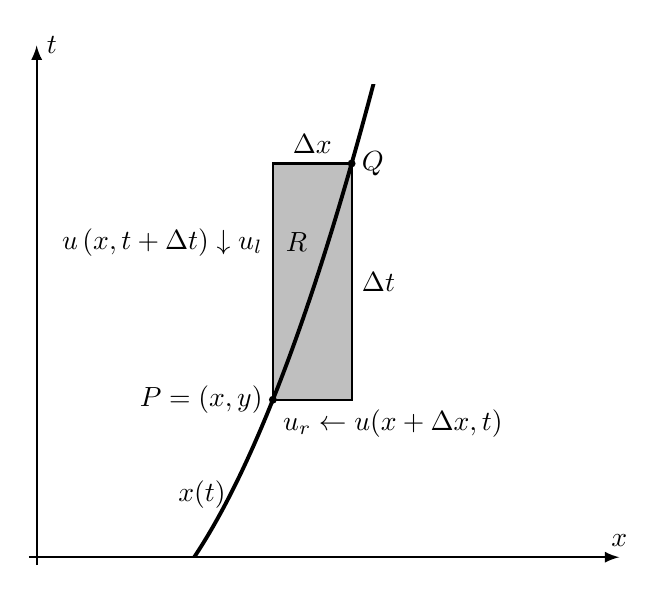
\begin{tikzpicture}[>=latex,thick]
\fill[color=gray!50] (3,2)--(4,2)--(4,5)--(3,5)--cycle;
\node at (3.3,4.0) {$R$};
\draw[->] (-0.1,0)--(7.4,0) coordinate[label={$x$}];
\draw[->] (0,-0.1)--(0,6.5) coordinate[label={right:$t$}];
\fill (3,2) circle[radius=0.05];
\node at (3,2) [left] {$P=(x,y)$};
\fill (4,5) circle[radius=0.05];
\node at (4,5) [right] {$Q$};
\draw (3,2)--(4,2)--(4,5)--(3,5)--cycle;
\node at (3.5,5) [above] {$\Delta x$};
\node at (4,3.5) [right] {$\Delta t$};
\begin{scope}
\clip (0,0) rectangle (7,6.0);
\draw[line width=1.4pt] plot[domain=2:5,samples=100] ({\x},{0.5*\x*\x -0.5*(\x)-1});
\end{scope}
\node at (3,4) [left] {$\begin{matrix}u(x,t+\Delta t)\\\downarrow\\u_l\end{matrix}$};
\node at (3,2) [below right] {$u_r\leftarrow u(x+\Delta x,t)$};
\node at (2.1,0.8) {$x(t)$};
\end{tikzpicture}
\caption{Herleitung der Hugoniot-Rankine-Bedingung für die Bewegung einer
Sprungstelle der Lösung eines Erhaltungssatzes.
\label{burgers:hugoniot}}
\end{figure}
In Abschnitt~\ref{subsection:nichtlineare} haben wir gesehen, dass Lösungen
der Gleichung von Burgers Sprungstellen entwickeln.
Die Formulierung als Erhaltungssatz in
Abschnitt~\ref{subsection:erhaltungssatz} 
soll uns jetzt erlauben, die Bewegung solcher Sprungstellen zu beschreiben.

Sie also $u(t,x)$ eine Lösung fast überall der Gleichung von Burgers mit
einer Sprungstelle, die sich entlangt der Kurve $x(t)$ bewegt.
Dazu berechnen wir das Wegintegral \eqref{burgers:integral} über den Rand
des Rechtecks mit den Ecken $(x,y)$ und $(x+\Delta x, y+\Delta y)$.
Wir benötigen die Grenzwerte
\[
\begin{aligned}
u_l &= \lim_{\Delta t\to 0+} u(t+\Delta t,x)
&&\text{und}&
u_r &= \lim_{\Delta x\to 0+} u(t,x+\Delta x).
\end{aligned}
\]
Damit können wir das Wegintegral approximieren als
\begin{align}
\int_{\partial R}(u\,dx -F(u)\,dt)
&=
0
\notag
\\
u(t+\Delta t,x)
\Delta x
-
F(u(t+\Delta t,x))
\Delta t
&=
u(t,x+\Delta x) \Delta x
-
F(u(t,x+\Delta x)) \Delta t
\notag
\\
\Delta x
(
u(t+\Delta t,x)
-
u(t,x+\Delta x)
)
&=
\Delta t
(F(u(t+\Delta t,x))
-
F(u(t,x+\Delta x))
)
\notag
\\
\intertext{Oder nach Grenzübergang $\Delta t\to 0$ und $\Delta x\to 0$}
\dot x(t)\, (u_l-u_r) &= F(u_l) - F(u_r).
\label{burgers:hugoniot-rankine}
\end{align}
Die Geschwindigkeit, mit der sich die Sprungstelle bewegt, hängt also 
von den Werten von $u(t,x)$ auf beiden Seiten der Sprungstelle ab.
Dies sind die {\em Hugoniot-Rankine-Bedingungen}.
Wir werden sie Abschnitt~\ref{burgers:training} verwenden, um Trainingsdaten
für Sprungstellen der Lösung zu erzeugen.
\index{Hugoniot-Rankine-Bedingungen}
\index{Rankine-Hugoniot-Bedingungen}


\subsection{Numerische Lösungen und Computational mode}
Bei der numerischen Lösung der Gleichung von Burgers tritt erschwehrend der
Computational Mode auf.


%
% burgertraining.tex -- Trainingsdaten für Burgers Gleichung
%
% (c) 2018 Prof Dr Andreas Müller, Hochschule Rapperswil
%
\subsection{Trainingsdaten für die Gleichung von Burgers}
Damit die Gleichung von Burgers mit einem Machine-Learning-Ansatz gelöst
werden kann, müssen geeignete Trainingsdaten bereitgestellt werden.


\subsubsection{Lösung mit Charakteristiken}

\subsubsection{Sprungstellen}



\printbibliography[heading=subbibliography]
\end{refsection}
